\cotefile{137}
\scanpage{59}
% archive sheet number: 58
\deleted{Il faut prouver que \deleted{le noyau} l'hom
\[
\operatorname{Hom}^{\bullet}_{k}(L^{\bullet},C)\longrightarrow Z^{n}(C^{\bullet})^{f}\subset (C^{n})^{f}
\]
a aussi un $\Sigma$-noyau}

\deleted{\diagram{\begin{tikzcd}[ampersand replacement=\&,column sep=small,row sep=small]
\& \underline{\mathrm{Hom}}_{\Sigma\text{-}\mathrm{sex}}\arrow[d] \& \&\\
\& B^{\bullet}\arrow[dl]\arrow[dr] \& \&\\
\underline{\mathrm{Hom}}_{\Sigma\text{-}\mathrm{ex}}\simeq B^{\mathrm{rés}}\arrow[dr] \& \& \deleted{\unsure{B^{\mathrm{plat}}}}\underline{\mathrm{Hom}}_{\mathrm{sex}}\arrow[dr] \&\\
\& B^{\unsure{\mathrm{rés.pl}|\mathrm{rés.ple}|\mathrm{rés}}} \& \& \deleted{\underline{\mathrm{Hom}}_{\mathrm{sex}}}B^{\unsure{\mathrm{plat}}}
\end{tikzcd}}
\margin{$\left.\vphantom{\begin{matrix}B\\B\\B\end{matrix}}\right\}$ $B$ cat. abélienne $\Sigma$ suites courtes ordinaires}}

\deleted{\[
\mathbb{E}\mathrm{xt}^{1}(L^{\bullet},M)\Longleftarrow 0
\]
\[
\underline{\mathrm{Hom}}_{\Sigma\text{-}\mathrm{ex}}(P,B)\xrightarrow{\approx}\underline{\mathrm{Hom}}_{\Sigma\text{-}\mathrm{lex}}(P_0,B)
\]
si $B$ \deleted{\illegible{2}} admet \unsure{(}$\inserted{\Sigma\text{-}}$noyaux}

\scanpage{60}
Cela signifie que l'on a une kyrielle de suites $\Sigma$-exactes (donc exactes)
\[
\begin{aligned}
0\longrightarrow\Psi^0\longrightarrow \mathbb{C}^0\longrightarrow\Psi^1\longrightarrow0&\\
\hspace{2em}0\longrightarrow\Psi^1\longrightarrow \mathbb{C}^1\longrightarrow\Psi^2\longrightarrow0&\\
\hspace{4em}0\longrightarrow\Psi^2\longrightarrow \mathbb{C}^2\longrightarrow\Psi^3\longrightarrow0&\\
&\cdots
\end{aligned}
\]
Par hyp on sait que
\[
\Psi^i_{\bullet}=k\ \text{placé en dim }i
\]
% slanted
\margin{\unsure{c'est peut-être pas a)|n'est-ce pas a)}}
On trouve aisément les \deleted{\unsure{Hom}$(\Phi$} \inserted{hom} entre les $\deleted{\Phi}\mathbb{C}^i$, et \deleted{\unsure{Hom}$(\,$les} $\Psi^j$
\[
\deleted{\Phi}\mathbb{C}^i\longrightarrow\Psi^j,\quad\Psi^i\longrightarrow\deleted{\Phi}\mathbb{C}^j,\quad\Psi^i\longrightarrow\Psi^j\qquad(\deleted{\Phi}\mathbb{C}^i\longrightarrow\deleted{\Phi}\mathbb{C}^j\ \text{déjà connu})
\]
on peut résumer la situation en disant que sur la sous-catégorie pleine $P_1\subset P$ formée des objets isom. à des sommes de $\Phi^i$ et de $\Psi^j$, le foncteur $L\longmapsto L_{\bullet}=\operatorname{Hom}(\Phi^{\bullet},L)$ est pl. fidèle. Son image essentielle est formée des complexes de chaînes $L_{\bullet}$ finis tels que les composantes \inserted{$L_i$, les $Z_i$ et les $B_i$} \deleted{\unsure{$H_i(L_{\bullet})$}} soient libres de \unsure{r. fi.|t. f.}

(On peut voir que le \deleted{\unsure{couple}} \inserted{\unsure{syst.}} $(P_1,\mathbb{C}^{\bullet},\Psi^0,\varepsilon,\Sigma\unsure{\cap|d}P_1)$ est universel pour les cat. $k$-additives munies d'une \deleted{\unsure{un}} \inserted{classe} $\Sigma$ de suites courtes, et d'une $\Sigma$-résolution d'un objet \deleted{$\Psi^0$}$Z^0$ \unsure{--|\ldots}).

On va maintenant supposer de plus

d) Pour tte suite \inserted{$\Sigma$-}exacte de $P$
\[
0\longrightarrow L^{\unsure{\flat|\bullet|0}}\longrightarrow M\longrightarrow N\longrightarrow0
\]
% slanted
\margin{il suffit d'avoir l'un des deux, p. ex. le \unsure{premier|récipr.}}
et tout hom $L\longrightarrow L'$ (resp $N'\longrightarrow N$) la suite \deleted{\unsure{som}} déduite par somme amalgam. (resp. produit fibré) existe dans $P$
% archive sheet number: 59

\scanpage{61}
et est $\Sigma$-exacte

(Variante: si $L\xrightarrow{u}M$ est \deleted{un $\Sigma$-épi} \inserted{\unsure{tel que|un}} \deleted{\unsure{alors il s'\illegible{1} aussi}} $\operatorname{Hom}(\Phi^i,u)$ est épi $\forall i$ (i.e. $u_{\bullet}:L_{\bullet}\longrightarrow M_{\bullet}$ épi) alors $u$ \deleted{\unsure{s'écrira}} admet un noyau (donc on a une suite $\Sigma$-exacte
\[
0\longrightarrow R\longrightarrow L\longrightarrow M\longrightarrow0\qquad)
\]

Utilisant ceci, on construit des objets de $P$ par ext. successives des objets $(\Psi_{\unsure{\varepsilon|i|\bullet}}^i)^{r_i}$ -- et on voit que $L\longmapsto L_{\bullet}=\operatorname{Hom}(\Phi^{\bullet},L)$ est un \uline{surjectif}.

e) Tout objet \inserted{$L$} de $P$ est extension successive d'objets de la forme $\Psi^i$ [qu'on peut supposer se suivre par ordre croissant, dans une filtration croissante \inserted{admissible} pour $P$ -- la quelle sera alors canonique.]

Il doit y avoir assez maintenant pour conclure que le foncteur $L\longmapsto L_{\bullet}=\operatorname{Hom}(\Phi^{\bullet},L)$ est ple. fid et a l'image essentielle les $L_{\bullet}$ tels que les $L_i$, $Z_i$, $B_i$, $H_i$ soient libres tf et \inserted{les $L_i$} nuls sauf un nb fini.
% archive sheet number: 60

\scanpage{62}
\uline{Remarque} Supposons $k$ principal. Alors la catégorie $P\simeq P_{\bullet}$ \deleted{\unsure{est ab.}} admet des \deleted{$\Sigma$} noyaux (et des Conoyaux, \deleted{\unsure{?|$\Sigma$}} mais un bimorphisme n'est pas néc. un iso). \deleted{\unsure{On fera attention que les mor.}} Il est \unsure{m.|il} vrai que si $N$ est le noyau de $A\longrightarrow B$, alors $N\longrightarrow A$ est un $\Sigma$-mono, i.e. s'insère dans une suite $\Sigma$-exacte $0\longrightarrow N\longrightarrow A\longrightarrow A'\longrightarrow0$, mais le mor. $A'\longrightarrow B$ ne sera pas en général un $\Sigma$-mono. \deleted{Aussi} On ne peut interpréter $(P,\deleted{\unsure{\Psi^0}}\mathbb{C}^{\bullet},\deleted{\unsure{\Psi^0,\varepsilon}}\inserted{\Sigma}\deleted{\unsure{,\Sigma}})$ comme sol. d'un pb universel en appliquant tels quels les développements précédents: \deleted{Mais \deleted{\unsure{disons}} \inserted{\unsure{on peut}} définir de façon naturelle, pour une $B$ $k$-linéaire, la notion d'objet \uline{plat}, et alors} le syst. ci-dessus est universel pour les $B$ \inserted{$k$-additifs} munis d'un complexe \deleted{de cochaînes \inserted{\unsure{libres}} plat, \deleted{\unsure{des}} d'un. \deleted{sys} \inserted{classe} $\Sigma$ de suites courtes, telles que tt hom $u\inserted{{}:A\longrightarrow B}$ de $B$ ait un noyau tel que $\operatorname{Ker}u\longrightarrow A$ soit $\in\Sigma$} $C^{\bullet}$ et d'une classe $\Sigma_C$ de suites exactes, telle que tt morphisme $u:A\longrightarrow B$ de \unsure{$\mathcal B$|$B$} admette un noyau $K$ tel que $K\longrightarrow A$ soit un $\Sigma_C$-mono: (on prend comme morphismes entre tels syst. ceux qui transforment $C^{\bullet}$ en $C'^{\bullet}$ et qui sont $\Sigma_{\unsure{i|1}}$-exacts à \uuline{g}).
% archive sheet number: 61

\scanpage{63}
On travaillera dorénavant dans la catégorie $P_1=Q$ (équivalente à la catégorie $Q_{\bullet}$ des complexes de chaînes finis où les \deleted{\unsure{-}} $L_i$, $Z_i$, $B_i$, $H_i$ sont libres de type fini), \inserted{munie de $\Sigma_1=\Sigma\cap P_1$,} dont la sous-catégorie des $\Sigma$-projectifs est \deleted{ad} la catégorie \inserted{additive} $P_0$ engendrée par les $\mathbb{C}^i$ et $\Psi^0$ (i.e. par les $\Phi^i$), et celle des $\Sigma$-injectifs est la sous-cat. additive $\mathbb{K}$ \deleted{\unsure{des faisceaux}} \inserted{engendrée} par les $\mathbb{C}^i$ (les $L_{\bullet}$ \deleted{flasques} acycliques i.e. les $L_*$ flasques --). \uline{On s'intéressera aux résolutions droites} \inserted{$K^{\bullet}$} $\Sigma$-\uline{injectives de} $\Psi^0$, (i.e. des résolutions flasques $K^{\bullet}_*$ de $k_*$ \unsure{$\simeq$} -- ce qui donneront, \inserted{du} en top algébrique \inserted{\unsure{$\simeq$}}, des méthodes de calcul remarquables de la coh à coeffs dans $k$). \unsure{On a|On a.} d'algèbre homologique ``relative'' \unsure{au choix de|au choix des|qui donne des} suites exactes, qui nous disent que si (comme c'est le cas ici) tout objet \deleted{\unsure{est q}} se plonge dans un $\Sigma$-injectif, \deleted{de façon} par un $\Sigma$-mono, alors \deleted{les} \deleted{les deux résolutions sont canoniquement \unsure{iso.}} deux résolutions sont homotopes, et il y a une seule classe d'homotopie d'hom de l'une dans l'autre (\uline{NB} Il y a aussi assez de projectifs, et on a l'assertion analogue pour les résolutions projectives; on fera attention que la cat. $\mathbb{K}$ des sommes de $\mathbb{C}^i$ \unsure{sera|bien|est}
% archive sheet number: 62

\scanpage{64}
contient pas \uline{assez} de \inserted{$\Sigma$-}projectifs; il faut y rajouter $\Psi^0$\ldots) \deleted{Il est vrai aussi} Ces \deleted{\unsure{mêmes}} assertions sont d'ailleurs valables aussi dans la plus gde catégorie $P$ [détermination des \inserted{$\Sigma$-}proj. et des $\Sigma$-inj. et le fait qu'il y en ait assez].

Les $\operatorname{Ext}^{i}$ calculés par les résolutions injectives \inserted{à droite}, ou projectives \deleted{\unsure{sont (à gauche}} \inserted{à g.} ou les deux simultanément, sont les \unsure{mê.|$\mathrm{Ext}$} pour $i\geq1$ ce sont les hyperext habituels de \inserted{$L_{\bullet}$ et de $M_{\bullet}$}, pour $i=0$ ce sont par contre les $Z^i$.

Si $F:Q=P_1\hookrightarrow P\longrightarrow B$ ($k$-add.) est un foncteur, on peut construire les foncteurs dérivés \inserted{à droite ou gauche} en utilisant des résolutions injectives ou projectives. Nous sommes intéressés notamment aux $R^iF(\Psi^0)$, qu'on notera aussi $H^i(F)$ [on doit pouvoir montrer que ce sont les dérivés \inserted{droits} de $F\longmapsto F(\Psi^0)\overset{\mathrm{déf}}{=}\Gamma(F)$, quand $F$ varie dans la cat. des foncteurs \inserted{$k$-add} $P\longrightarrow \underline{B}$ \inserted{$\Sigma$-}exacts à gauche, (si on se restreint à de tels $F$); qu'en effet cette catégorie est équivalente: \deleted{\unsure{del.}} $\deleted{\unsure{B}} B^{\bullet}$, $F\longmapsto F(\Psi^0)$ s'identifie, \deleted{\unsure{alors}} foncteur $C^{\bullet}\longmapsto Z^0(C^{\bullet})\inserted{{}=H^0(C^{\bullet})}$ sur $B^{\bullet}$, dont les dérivés sont comme sont les $H^i(C^{\bullet})$ pour $i\geq1$. On a aussi $RF(\Psi^0)\simeq F(\mathbb{C}^{\bullet})$
% archive sheet number: 63

\scanpage{65}
(iso dans cat. dérivée) puisque $\mathbb{C}^{\bullet}$ est une résolution $\Sigma$-injective de $\Psi^0$.

\figure{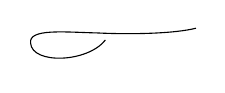
\begin{tikzpicture}[x=1cm,y=1cm]\draw (0.75,0.02) .. controls (0.52,-0.27) and (-0.18,-0.29) .. (-0.2,-0.02) .. controls (-0.23,0.17) and (0.23,0.12) .. (0.65,0.11) .. controls (1.07,0.09) and (1.62,0.1) .. (1.9,0.17);\end{tikzpicture}}

Nous considérons maintenant les réalisations $\frac12$ simpliciales $P_*\supset Q_*\supset \deleted{\unsure{Q}}P_{0*}\supset \mathbb{K}_*$ \deleted{\unsure{$Q$}} de $P\supset Q\supset \deleted{\unsure{Q}}P_0\supset\mathbb{K}$. Or sur \deleted{\unsure{la}} $P_*$ il y a la structure $\otimes_{\deleted{\unsure{\Sigma}}*}$ ou $\otimes_*$ ($L_*\otimes_*M_*$ défini \unsure{composantes par composantes|composante par composante}
\[
(L_*\otimes M_*)_{[n]}=L_{[n]}\otimes M_{[n]}\qquad)
\]
avec contraintes d'ass, unité ($\Psi^0$), et de comm., \inserted{$\otimes$ du bilex.} \deleted{\unsure{De même que la réalisation (contravariante) $P^*,Q^{\bullet}$,|De même que la réalisation (contravariante) $P^*,Q^*$,}} On note que $\mathbb{K}_*$ est un ``idéal'', i.e. que \deleted{\unsure{l'on est un des facteurs}} \inserted{\unsure{lire|i.e.}} si un des facteurs $L_*,M_*$ est dans $\mathbb{K}_*$, l'autre aussi), $P_0$ et $Q$ sont stables par $\otimes$, car
% slanted
\margin{\deleted{\unsure{et}} il n'y a pas de \uline{Hom} interne mais on a \unsure{certaines (dualités)|aussi un (des Ext)}}
\[
\begin{aligned}
\Psi^0_{\unsure{\bullet|0}*}\otimes\Psi^0_{\bullet*}&\simeq\Psi^0_{\bullet*}\quad(\Rightarrow\text{ stabilité de }\unsure{\mathcal G|\mathbb{K}|P_0})\\[-.3ex]
\underset{\mathbb 1_*}{\Vert}\hspace{1.7em}\underset{1_*}{\Vert}&\hspace{1em}\underset{\mathbb 1_*}{\Vert}
\end{aligned}
\]
et
\[
\begin{aligned}
\Psi^i_*\otimes\Psi^j_*&\simeq\Psi^{i+j}_*+\text{ élément de }\mathbb{K}\\
&(\Rightarrow\text{ stabilité de }P_{1*}=\unsure{Q'|Q})
\end{aligned}
\]

On transporte cette structure multiplicative sur $P$ et ses sous-catégories (notation $*$, pour éviter des confusions) et ses autres réalisations $P_{\bullet}$ et $P^{*}$, $P^{\bullet}$ (ces deux dernières \unsure{contragrédientes|contravariantes}). On note $*$ sur $P_{\bullet}$ et $P^{\bullet}$, et $\otimes$ ou $\overset{*}{\otimes}$ sur $P^{*}$, car l'équivalence des
% archive sheet number: 64

\scanpage{66}
$P_*$ avec $P^*$ est compatible au $\otimes$.

Soit $B$ une cat. ($k$-)additive avec op. ($k$-)bil. $\otimes$ \inserted{(propriété des foncteurs \deleted{$\otimes$})} \uline{\unsure{muni|munie}} d'une contrainte d'ass, d'unité, et de comm. \inserted{(données)} \deleted{\unsure{tels}} satisf. aux compatibilités habituelles (propriété). Soit $B'$ une autre telle. Si on a un foncteur ($k$-)additif (propriété)
\[
F:B'\longrightarrow B
\]
on appelle \uline{structure multiplicative sur $F$} \unsure{tout|deux} hom de \inserted{bi}foncteurs
\[
F(X)\otimes F(Y)\xrightarrow{u_{X,Y}}F(X\otimes Y)
\]
et un \unsure{hom|iso} $\deleted{\unsure{F(1)\longrightarrow}}\,\mathbb 1_B\xrightarrow{\alpha}F(\mathbb 1_{B'})$ qui soient compatibles aux données d'ass., d'unité de comm.

\diagram{\begin{tikzcd}[ampersand replacement=\&,column sep=large,row sep=large]
(F(X)\otimes F(Y))\otimes F(Z)
 \arrow[r,"{\deleted{\unsure{u}}\;u_{X,Y}\otimes F(Z)}"] \arrow[d,"{\sim}"',"{a^B_{F(X),F(Y),F(Z)}}"]
 \& F(X\deleted{\unsure{)}}\otimes Y)\otimes F(Z)\arrow[d,"{u_{X\otimes Y,Z}}"] \\
F(X)\otimes(F(Y)\otimes F(Z))\arrow[d,"{F(X)\otimes u_{Y,Z}}"']\arrow[r,phantom,"\mathrm{comm}"]
 \& F((X\otimes Y)\otimes Z)\arrow[d,"{\sim}"',"{F(a^{B'}_{X,Y,Z})}"]\\
F(X)\otimes F(Y\otimes Z)\arrow[r,"{u_{X,Y\otimes Z}}"'] \& F(X\otimes(Y\otimes Z))
\end{tikzcd}}

\diagram{\begin{tikzcd}[ampersand replacement=\&,column sep=large,row sep=small]
F(X)\otimes\mathbb 1_B\arrow[r,"{F(X)\otimes\alpha}"]\arrow[ddr,"{\delta^B_{F(X)}}"',"{\sim}"] \& F(X)\otimes F(\mathbb 1_{B'})\arrow[d,"{u_{X,\mathbb 1_{B'}}}"]\\
{}\arrow[r,phantom,"\mathrm{comm}"] \& F(X\otimes\mathbb 1_{B'})\arrow[d,"{\sim}"',"{F(\delta^{B'}_X)}"]\\
\& F(X)
\end{tikzcd}}
\margin{et symétrique}

\diagram{\begin{tikzcd}[ampersand replacement=\&,column sep=large]
F(X)\otimes F(Y)\arrow[r,"{u_{X,Y}}"]\arrow[d,"{\sigma^B_{F(X),F(Y)}}"']\arrow[dr,phantom,"\mathrm{comm}"] \& F(X\otimes Y)\arrow[d,"{F(\sigma^{B'}_{X,Y})}"]\\
F(Y)\otimes F(X)\arrow[r,phantom,"{\overset{u_{Y,X}}{\unsure{\relbar|\longrightarrow}}}" description] \& F(Y\otimes X)
\end{tikzcd}}
% archive sheet number: 65

\scanpage{67}
NB $F(\mathbb 1_{B'})$ \unsure{devient alors|devra être|devient donc} un ``objet-\deleted{($k$)}anneau'' de $B$ (``$k$-Algèbre'' quand il y a un $k$) $F$ transforme ``anneaux'' de $B'$ en ``anneau'' de $B$, en respectant les \unsure{propr.|proprs} d'unité, associativité ou commutativité.

Les $F$ en question forment une catégorie. Si on a $B''$, $B'$, $B$, ils se composent, d'où $2$-catégorie des $\otimes$-catégories $k$-additives.

\uline{Supposons maintenant que} $B'=\mathbb{K}$ -- (catégorie dans laquelle se trouvent ttes nos résolutions injectives --). Un foncteur $k$-lin.
\[
\mathbb{K}\xrightarrow{F}B
\]
s'identifie alors à un $C\in B^{\bullet}$. Donc on sait ce qu'il faut entendre par ``structure multiplicative sur le complexe de cochaînes $C^{\bullet}$'' de $B^{\bullet}$ (on dira: str. mult. demi-simpliciale'' pour ne pas prêter à confusion).
% archive sheet number: 66

\scanpage{68}
Comme, \uline{donnée}, c'est un hom de bifoncteurs
\[
F(X)\otimes\deleted{\unsure{*}}F(Y)\longrightarrow F(X\deleted{\otimes}*Y)
\]
or il suffit de \deleted{\unsure{le}} le donner sur la sous catégorie \inserted{\unsure{de la|$k$-lin.}} $\Delta\times\Delta$ \inserted{de $\mathbb{K}\times\mathbb{K}$} des $\mathbb{C}^i\times \mathbb{C}^j$, (avec sa structure \unsure{$k$-lin|bi-lin}) donc de se donner des hom de bicomplexe de cochaînes
\[
\underset{C^{\bullet}}{\underset{\Vert}{F(\mathbb{C}^{\bullet})}}\otimes_B
\underset{C^{\bullet}}{\underset{\Vert}{F(\mathbb{C}^{\bullet})}}\longrightarrow
F(\deleted{\unsure{\Phi}}\mathbb{C}^{\bullet}*\deleted{\unsure{P}}\mathbb{C}^{\bullet})\quad\text{dans } B^{\bullet\bullet}
\]
ce qu'on \unsure{peut encore|pourrait|peut} expliciter, si $\mathbb{C}^i\deleted{\otimes}*\mathbb{C}^j$ correspond au bicomplexe de chaînes \inserted{\unsure{flasques de|défini par}} $\mathbb{C}^i_{\bullet}*\mathbb{C}^j_{\bullet}=\deleted{\unsure{C^i_{\bullet}\otimes}}\operatorname{ND}_{\bullet}(\underset{\bigwedge^{i+1}\Phi_*\otimes\bigwedge^{j+1}\Phi_*}{\underset{\Vert}{\mathbb{C}^i_*\otimes \mathbb{C}^j_*}})$
% slanted
\margin{cas le plus commun: $B=\unsure{\mathit{Ab}_k|\mathit{Ab}}$}
\[
\underset{C^i}{\underset{\Vert}{F(\mathbb{C}^i)}}\otimes_B
\underset{C^j}{\underset{\Vert}{F(\mathbb{C}^j)}}\longrightarrow
\operatorname{Hom}^{\bullet}_k\bigl(\underset{C_i^{\bullet}\deleted{\otimes}*C_j^{\bullet}}{\underset{\Vert}{(\mathbb{C}^i_{\bullet}*\mathbb{C}^j_{\bullet})^{\vee}}},C^{\bullet}\bigr)
\tag*{1)}
\]
i.e.
\[
(C^i_{\unsure{\xi|\zeta}}\otimes_B C^j)\otimes_k
\underbrace{\overbrace{(C_i^{\bullet}*C_j^{\bullet})}^{\mathrm{déf}\ \Vert\ C^{\bullet}_{i,j}\deleted{\unsure{N}}}}_{\in\mathbb{K}^{\bullet}}\longrightarrow C^{\bullet}
\tag*{2)}
\]
avec compatibilité aux op. diff. pour $i,j$ variables.

On peut aussi l'écrire
\[
\deleted{(C^i\otimes_B C^j)\otimes_k}
\]
\[
C^i\otimes_B C^j\longrightarrow
\operatorname{Hom}^{*}_{k}(\underbrace{C_i^*\otimes C_j^*}_{\bigwedge^{i+1}\Phi^*\otimes\bigwedge^{j+1}\Phi^*},\underset{\operatorname{DP}^*(C^{\bullet})}{\underset{\Vert}{C^*}})
\tag*{(1*)}
\]
ou encore
\[
(C^i\otimes_B C^j)\otimes_k
\underbrace{\bigl(\bigwedge^{i+1}\underline{\Phi}^{*}\overset{*}{\otimes}\bigwedge^{j+1}\underline{\Phi}^{*}\bigr)}_{C_{i,j}^{*}\unsure{\simeq}\,}
\xrightarrow{u^{i,j}}C^{*}
\tag*{(2*)}
\]
% archive sheet number: 67

\scanpage{69}
hom \unsure{compatible|compatibles} aux op. $\frac12$ simpliciales (pour $i,j$ \unsure{fixé|fixés}) et les op. diff (pour $i,j$ \unsure{variable|variables})
\diagram{\begin{tikzcd}[ampersand replacement=\&,column sep=huge,row sep=large]
C^i\otimes_B C^j)\otimes C_{ij}^{*\deleted{\unsure{n}}}\arrow[d] \& C^i\otimes_B C^j)\otimes C_{i+1,j}^{*\unsure{n}}\arrow[l,"{d^{\unsure{k0|k\circ|*}}_{i+1,j}}"']\arrow[d,"{d^i\otimes-\otimes-}"]\\
\deleted{\unsure{C^i\otimes C^j\otimes C^*_{ij}}}\ C^* \& \deleted{\unsure{\leftarrow(C^{i+1}\otimes_B C^j)\otimes C^{*}_{i+1,j}}}\ (C^{i+1}\otimes_B C^j)\otimes C_{i+1,j}^{*\unsure{,j}}\arrow[l,"{d_{\bullet}}"]
\end{tikzcd}}

plus des données de compatibilités -- avec unité, assoc, comm. (\unsure{la dernière|les dernières|Elles devraient} s'\unsure{explicitant|explicitent|explicite|expliciter} de façon particulièrement triviale).

\uline{Remords} $\mathbb{K}$ n'a pas d'unité pour $*$! donc \deleted{\unsure{il}} on ne peut exprimer directement, en restant dans $\mathbb{K}$, une compatibilité avec les \deleted{unités}\unsure{unités}! Comment s'en tirer? Si on passe à $P_0$ ou $Q=P_1$, \deleted{\unsure{on a} \illegible{2} d'une famille $\Sigma$ de suites courtes,} on trouve que les foncteurs $k$-additifs de $\deleted{\unsure{P}}Q$ (resp. $P_0$) dans $B$ qui sont $\Sigma$-exacts à gauche (i.e. transforment des \inserted{$\Sigma$-}suites exactes courtes $0\longrightarrow A'\longrightarrow A\longrightarrow A''\longrightarrow0$ en suites ex à $0\longrightarrow F(A')\longrightarrow F(A)\longrightarrow F(A'')$) \deleted{avec $F(A')\longrightarrow F(A)$ un $\Sigma$-mono} correspondent par $F\longmapsto F(\mathbb{C}^{\bullet})$ aux complexes de coch dans $B$ tels que $\forall i$ (resp \unsure{pour}
% archive sheet number: 68

\scanpage{70}
$i=0$ seulmt) $C^i\xrightarrow{d^i}C^{i+1}$ ait un Ker \deleted{qui soit tel que $Z^i\longrightarrow C^i$ soit un $\Sigma$-mono (Ici, le $\Sigma$ dans $B$ est de la \unsure{poudre} aux yeux, il n'y a \unsure{à y penser}).} Ceci dit, on se borne à de tels complexes, qui correspondent donc à des foncteurs \deleted{\unsure{$\Sigma$-$P$}} $k$-add. \inserted{($\Sigma$-ex. à g)} $P_0\longrightarrow B$ resp. $Q\longrightarrow B$. \deleted{On se propose de \inserted{\unsure{se}} donner une structure multiplicative sur ceux-ci, ce qui nous oblige à donner de plus
\[
\deleted{F(\Psi^0)\otimes_B F(\mathbb{C}^i)\longrightarrow F(\Psi^0*\mathbb{C}^i)\text{ et }\unsure{\mathrm{sym}}}
\]
hom de bifoncteurs
\[
F(X)\otimes_B F(Y)\longrightarrow F(X*Y)
\]
sur $P_0\times P_0$ resp $Q\times Q$. Or \unsure{$P$}}

Si \unsure{enfin|même|tout} dans $B$ tte flèche a un noyau, alors on se bornera aux foncteurs $\Sigma$-ex. à g de $P$ dans $B$, en \deleted{\unsure{prolongeant}} interprétant ceux-ci comme des foncteurs $k$-additifs quelconques sur $\mathbb{K}$ i.e. des $C^{\bullet}\in\mathrm{ob}\,B^{\bullet}$. On peut l'expliciter ainsi: tt $L\in P$ \inserted{($\in Q,\in P_0$} \deleted{\unsure{(ou soit}} s'insère dans \deleted{deux} $\Sigma$-suites de $P$ ($Q,P_0$)
\[
\begin{aligned}
0\longrightarrow L\longrightarrow \unsure{I|\mathbb I}'\longrightarrow L'\longrightarrow0&\\
&0\longrightarrow L'\longrightarrow J^{\unsure{''|'}}\longrightarrow L''\longrightarrow0
\end{aligned}
\]
avec $I,J'\in\mathbb{K}$, et par suite en
% archive sheet number: 69

\scanpage{71}
Calculer $F$ à l'aide de sa restriction à $\mathbb{K}$ comme
\[
F(X)\simeq\unsure{\mathbb R|R}^0F(L)\simeq\operatorname{Ker}(F(I)\longrightarrow F(J))
\]
Ceci dit, \deleted{\unsure{si}} on a
\diagram{\begin{tikzcd}[ampersand replacement=\&,column sep=large]
F(X)\otimes_B F(Y)\arrow[r,"{?}"]\arrow[d] \& F(X*Y)\arrow[d]\\
F(I)\otimes_B F(J)\arrow[r,"{\substack{\text{connu}\\\text{par } F\vert\mathbb{K}\ \text{et sa}\\\text{structure mult.}}}"'] \& F(I*J)
\end{tikzcd}}

Or on voit que \deleted{si} $*$ transforme des couples de $\Sigma$-monos en un $\Sigma$-mono (résulte immédiatement des formules de Dold Puppe) donc la $2^{\text{ème}}$ flèche verticale est un mono d'où la détermination unique de ?. (Le fait qu'il soit indépendant des choix faits est immédiat, et aussi qu'il satisfait aux compatibilités d'ass. et de comm. si sa restriction à $\mathbb{K}$ y satisfait. Il reste donc à examiner l'axiome d'unité, \deleted{qui est que} il faut donc se donner
\[
\deleted{F(\Psi_0)}\mathbb 1_{B'}\longrightarrow F(\Psi_0]\xrightarrow{\sim}Z^0(C^{\bullet})
\]
et on voit que l'axiome signifie que c'est une \uline{unité} pour la structure de ``$k$-$\otimes$-Alg'' de $F(\deleted{\unsure{\Phi}}\Psi^0)$ (qui est une ``$k$-$\otimes$-Alg ass. comm'' \unsure{de tte}).
% margin note written sideways
\margin{\uline{NB} Donc on voit qu'on n'a pas besoin de l'existence de $\operatorname{Ker}(d^0:C^0\longrightarrow C^1)$ il suffit de dire qu'on donne $\mathbb 1_B\longrightarrow C^0$ dont le composé avec $C^0\longrightarrow C^1$ est nul, et qui joue le rôle d'une unité \deleted{\unsure{de $F(C^0$}} en un sens qu'on \unsure{explicitera|conjecture}}
% archive sheet number: 70

\scanpage{72}
\uline{Application} Toutes les constructions (``universelles'') dans $P_*^{\unsure{2|\Sigma}}$ \deleted{qui} (ou $\deleted{\unsure{P}}Q_*^{\unsure{1}},P_{0*},\mathbb{K}_*$) qui se font \unsure{uniquement|intrinsèquement} en termes de sa structure $k$-lin et sa $\otimes$-structure, \deleted{donnent} \inserted{se reflètent en} des constructions analogues sur un $C^{\bullet}\in\mathrm{ob}\,B^{\bullet}$ muni de structure multiplicative.

\uline{Ex 1} \deleted{\unsure{1 $\mathbb{C}^{\bullet}_*$ On a un hom|$\Psi^0$ $\mathbb{C}^{\bullet}_*$ On a un hom}} \inserted{Comme} $\mathbb{C}^{\bullet}_*\otimes \mathbb{C}^{\bullet}_*$ est une résolution $\Sigma^{\unsure{*}}_*$-inj. de $\Psi^0_{\unsure{\bullet|0}*}$ dans $P_{0*}$ tt comme $\mathbb{C}^{\bullet}_*$ lui-même on trouve
\[
\underset{\substack{\downarrow\\\unsure{\substack{\text{complexe}\\\text{simple associé}}|\substack{\text{avec les}\\\text{signes usuels}}}}}{\operatorname{Tot}^{\bullet}}(\mathbb{C}^{\bullet}_*\deleted{\unsure{\ast}}\otimes \mathbb{C}^{\bullet}_*)\longrightarrow \mathbb{C}^{\bullet}_*\quad\text{défini à homotopie}
\]
près, d'où un hom
\diagram{\begin{tikzcd}[ampersand replacement=\&,column sep=large,row sep=small]
F_{C^{\bullet}}(\mathbb{C}^{\bullet}_*\deleted{\unsure{\otimes}}*\mathbb{C}^{\bullet}_*)\arrow[r] \& F(\mathbb{C}^{\bullet}_*)\arrow[d,equal]\quad\text{défini à hom. près}\\
F_{C^{\bullet}}(\mathbb{C}^{\bullet})\otimes_B F_{C^{\bullet}}(\mathbb{C}^{\bullet})\arrow[u] \& C^{\bullet}\\
\mathbb{C}^{\bullet}\otimes C^{\bullet}\arrow[u,equal] \&
\end{tikzcd}}
d'où en composant un hom défini à homotopie près
\[
C^{\bullet}\otimes_B C^{\bullet}\longrightarrow C^{\bullet}
\]
avec conditions d'associativité, de comm. (attention aux signes!) et d'unité -- le tout à homotopie près. Il en résulte une structure de ``$\otimes B$ Alg. \unsure{graduée|gradué}'' sur $H^*(C^{\bullet})$, avec les propriétés habituelles.
% archive sheet number: 71
